\documentclass[output=paper]{langsci/langscibook}
\ChapterDOI{10.5281/zenodo.573788}

\author{Wendy Sandler\affiliation{University of Haifa}}
\title{What comes first in language emergence?} 
% \abstract{} 
\maketitle
\begin{document}
% \todo{who owns the rights for the images used? Do we have permission to publish them as CC-BY?}
 
\is{language evolution} \is{syllables} \is{syntax} \is{holophrases} \is{musical protolanguage} \is{syntactic recursion} \is{discrete infinity} \noindent There has been much speculation about what came first in the evolution of human language -- repetitive syllables that took on meaning \citep{MacNeilage1998} or that provided a structural basis for syntax \citep{Carstairs-McCarthy1999}; words \citep{Bickerton1990,Jackendoff1999}; undecomposable holophrases (e.g., \citealt{Arbib2012}); or musical protolanguage (\citealt{Darwin1871,Fitch2010}; see \citealt{Newmeyer2002} and \citealt{Fitch2005} for informative overviews).\footnote{Some theorists have proposed that spoken language emerged from gesture \citep{Corballis2002,Armstrong1995,Arbib2012}. I do not deal with that issue here, but see also e.g., \citet{MacNeilage1998}; and \citet{Sandler2013}; \citet{Emmorey2013}; and other papers in \citet{Kemmerer2013} for discussion.  }  Others have argued that the defining property at the evolutionary core of the human language faculty is syntactic recursion \citep{Hauser2002}, more recently described as a computational operation combining and recombining linguistic units \citep{Bolhuis2014}, or ``discrete infinity" \citep{Hauser2014}.  Whatever one takes to have been fundamental, it is reasonable to assume that language must have evolved in stages, and that, in some cases, the emergence of one property must have depended on another that preceded it, in the sense that it could not have evolved without it. 

\is{sign languages} It is difficult to support, refute, or flesh out hypotheses about these stages of evolution with evidence from spoken languages alone, because they are all thousands of years old, or descended from old languages, with their full linguistic structure intact.  However, sign languages can arise anew at any time, and linguists look to them for clues to the course of language emergence.  

\is{sign languages} \is{sign languages!new} The fact that the emergence of sign languages can be observed in real time does not guarantee that they will provide clues to the course of evolution of the human language capacity.  If these young sign languages were to make their appearance replete with complex linguistic structures, they would be of little help in determining how such structure emerged in evolution.  It is only if they develop gradually, and if the stages in this process can be identified, that they might offer concrete contemporary evidence of the path of language emergence.  

\is{prosodic organization} Here I will identify such evidence in a new sign language that arose in relative isolation, to show that modest linguistic machinery – holistic words and prosodic organization of semantically related words – are the first things to emerge, and that they are enough to support fully functional language.  Other, more computational, aspects of linguistic form, such as phonological, morphological,\footnote{Sign languages in general have certain types of modality-typical complex morphology (e.g., \citealt{Aronoff2005}).  We were surprised not to have found this complexity at the morphological level in Al Sayyid Bedouin Sign Language, although the beginnings of a system can be discerned in compounds.  See \citet{Meir2010} and \citet{Padden2010} for treatments of the emergence of morphology in ABSL. } and syntactic structuring, are later arrivals, apparently requiring the prior scaffolding provided by simplex words and by prosodic constituents that temporally organize semantically related units and characterize them with intonation.\footnote{I am assuming here that prosody includes intonation as well as rhythm (timing) and stress.}  

\is{sign languages!new} \is{language evolution} Of course, it cannot be assumed that the emergence of new sign languages in biologically modern humans faithfully replicates the evolution of language in our species.  But the modernity of these languages does not nullify their significance in the context of evolution, and it would be a mistake to dismiss them.  Emerging sign languages offer an exciting opportunity to identify two central facets of language emergence that no other naturally occurring system can provide.  One is the nature of the communicative elements that are required minimally in order for a system to function as language.  The other facet, relevant for the theme of this volume, is the path along which one kind of structure follows, or is dependent on, another over time before arriving at the kind of rule governed complexity in language that we often take for granted.  In this sense, new sign languages can offer a uniquely empirical and plausible reference point for models of language evolution.   

\is{sign languages!new} New sign languages have a heuristic advantage over spoken languages in another way as well.  The nature of the physical system, in which movements of different parts of the body (the two hands, the head, the face, the torso) visually manifest different linguistic functions, makes it possible for linguists to match form to function more directly than they can for spoken languages, and literally to see it unfold \citep{Sandler2012a}.  I refer to this correspondence between the recruitment of articulators for linguistic purposes and language form as the Grammar of the Body. \is{grammar of the body}

\newpage 
Investigation of \ili{Al-Sayyid Bedouin Sign Language} (ABSL), a young sign language that arose in relative isolation, has shown that a language does not spring forth fully formed, but rather evolves gradually across generations (see \citealt{Aronoff2008}; \citealt{Sandler2014handbook} for overviews).\footnote{As Keren Rice pointed out to me, no criteria are offered for measuring whether language emergence is gradual or abrupt, and indeed, the characterization depends a lot on one’s expectations.  Coming from the generative tradition that attributes a fair amount of linguistic structure to innate propensities, our group was surprised by the lack of much linguistic structure in the early stages of ABSL, and by the seemingly arduous path to its accrual and conventionalization, leading us us to characterize emergence of linguistic form as gradual.  For an overview of our ABSL findings, see \citealt{Sandler2014handbook}.}  Studying this language in different age groups, and tracing the step-by-step recruitment of different articulators to create a linguistic system \citep{Sandler2012a}, allows us to observe the gradual emergence of linguistic form over time. 

\is{word order} \is{human vs. inanimate} Our data suggest that language develops very efficiently, first, by creating holistic units to signify concepts -- words with no phonology.   This is followed by combining words into short propositions and later into larger discourse units, and organizing them prosodically into a fully functional linguistic system.  Word order comes in early as well \citep{Sandler2005}, although we now have reason to believe that it is determined by the fundamental opposition between human and inanimate referents, and not by syntax \citep{MeirSubmitted}. 

\is{meaningful vs. meaningless} \is{duality of patterning} \is{prosody vs. syntax} \is{conventionalization} \is{interactional linguistics}I will extrapolate from our findings on \ili{Al-Sayyid Bedouin Sign Language} to propose that certain basic elements of language must be present before other components commonly thought of as fundamental can arise.  First, the crystallization of phonology depends on conventionalization of lexical items, which in turn depends on repeated social interactions with the same social group.  These factors lead to automaticity, which results in a split between form and meaning. This split paves the way for duality of patterning \citep{Hockett1960} -- meaningful and meaningless (phonological) levels of structure.  The second two related properties are prosody and syntax.  In ABSL, prosodic structure organizes semantic relations in the absence of concrete evidence for any syntactic means of marking the same relations.  With little evidence for syntax in ABSL, I conclude that syntactic structure is not a prerequisite for the emergence of prosodic organization. 

\largerpage[-2]
\is{phonology} \is{autonomous syntax} The pattern of emergence we see suggests that central properties of language that are considered universal – phonology and autonomous syntax -- do not come ready-made in the human brain, and that a good deal of language can be present without clear evidence for them.  I begin with a snapshot of the Grammar of the Body in established sign languages to show how linguistic structure manifests itself in these visual languages\footnote{For comprehensive treatments of sign language linguistic structure at all levels, see \citet{Sandler2006} and \citet{Pfau2012}.     }, and then go on to emergence.{ }

\section{The Grammar of the Body}

\is{grammar of the body} \is{sign languages} Sign languages are sometimes described as manual languages because the hands convey words, the most essential linguistic units.  But sign languages also systematically exploit the whole upper body to convey language:  movements of the head, facial articulators, and the torso, and independent use of the nondominant hand.  Different movements of the extra-manual bodily articulators individually and in combination convey important elements of structure, including subordination, adjectival- or adverbial-type modification, contrast, intonation, and more, as shown in \figref{fig:sandler:3} below.\footnote{There is a large literature on nonmanual linguistic use of the body in sign languages.  See \citet{Pfau2010}, \citet{Sandler2012b}, and a special issue of \textit{Sign Language and Linguistics }(2011), Hermann and Steinbach (Eds.).}  The two levels to be traced here are the word and prosody/intonation.  

\is{sign languages!established} \is{phonology} In established sign languages, words have phonological structure: different configurations of the fingers, orientations of the palm, and movements of the hand on or near different body locations are combined to create signs and to distinguish them from one another, and they are altered in phonological processes such as assimilation \citep{Stokoe1960,Sandler1989,Liddell1989,Brentari1998}.  \figref{fig:sandler:1} shows a minimal pair in \ili{Israeli Sign Language} (ISL) distinguished by differences in major place of articulation alone.

\begin{figure}
{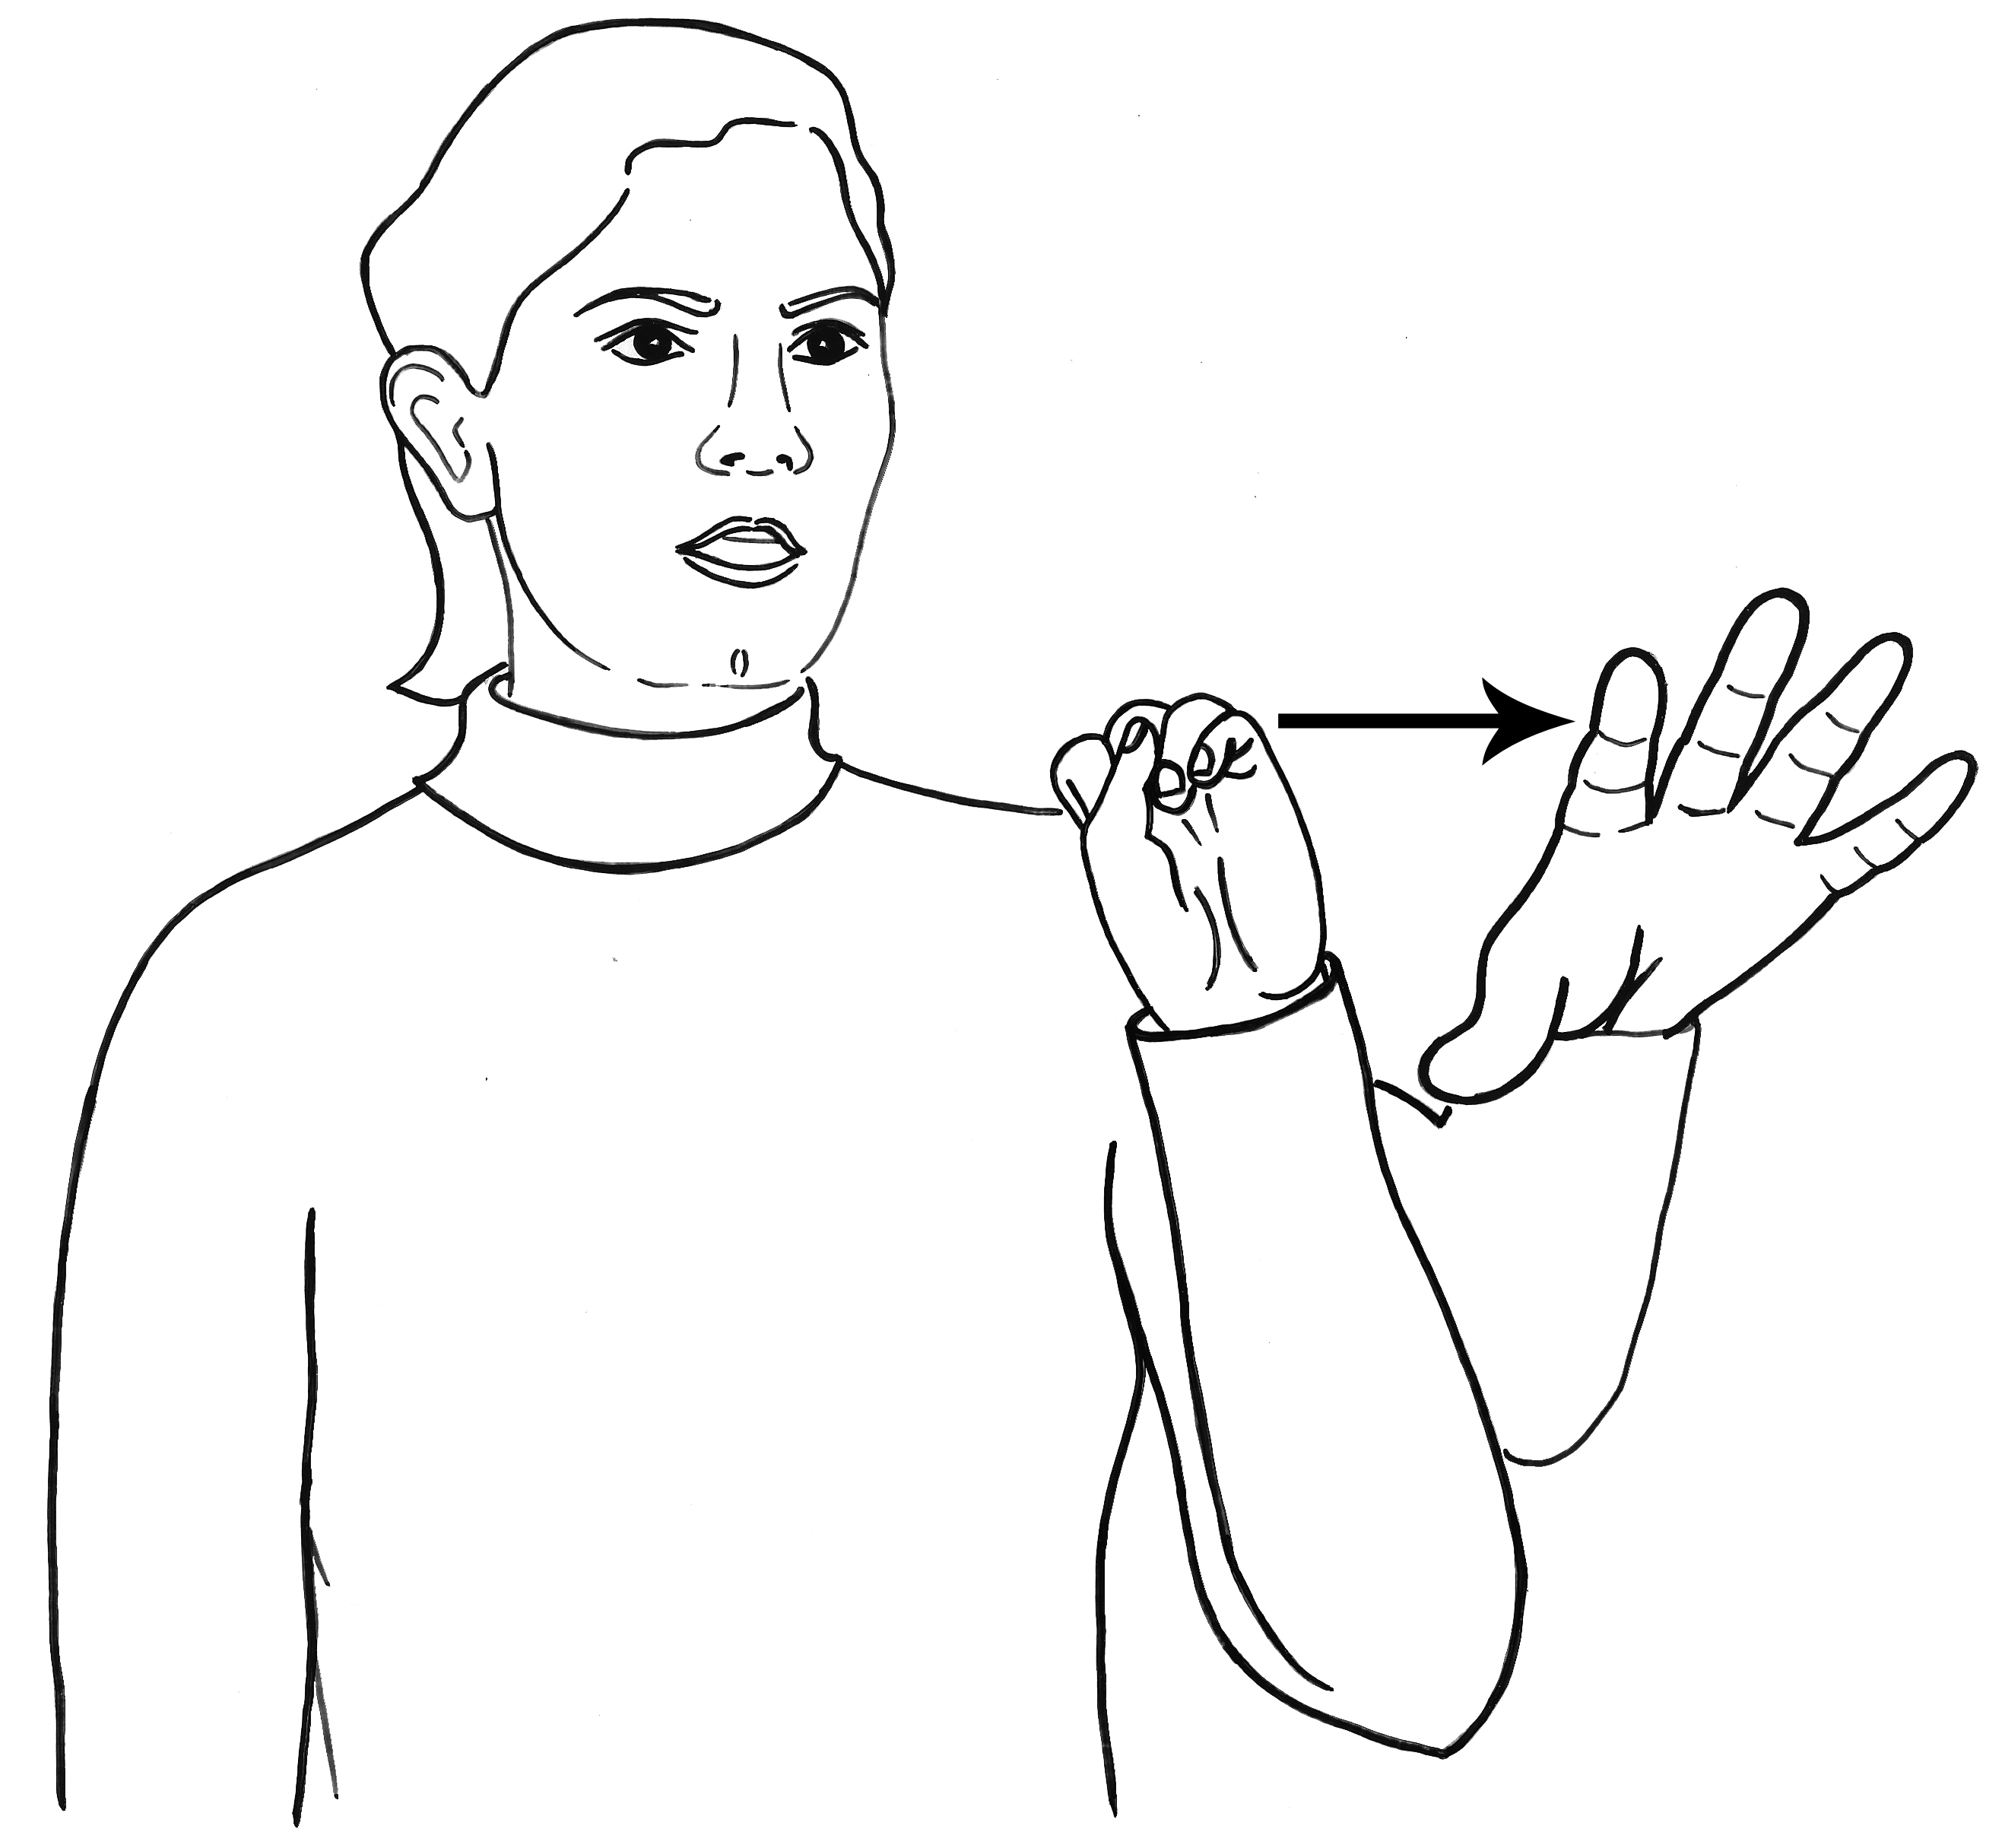
\includegraphics[width=0.38\textwidth]{figures/1a__SEND_copy.jpg}}
{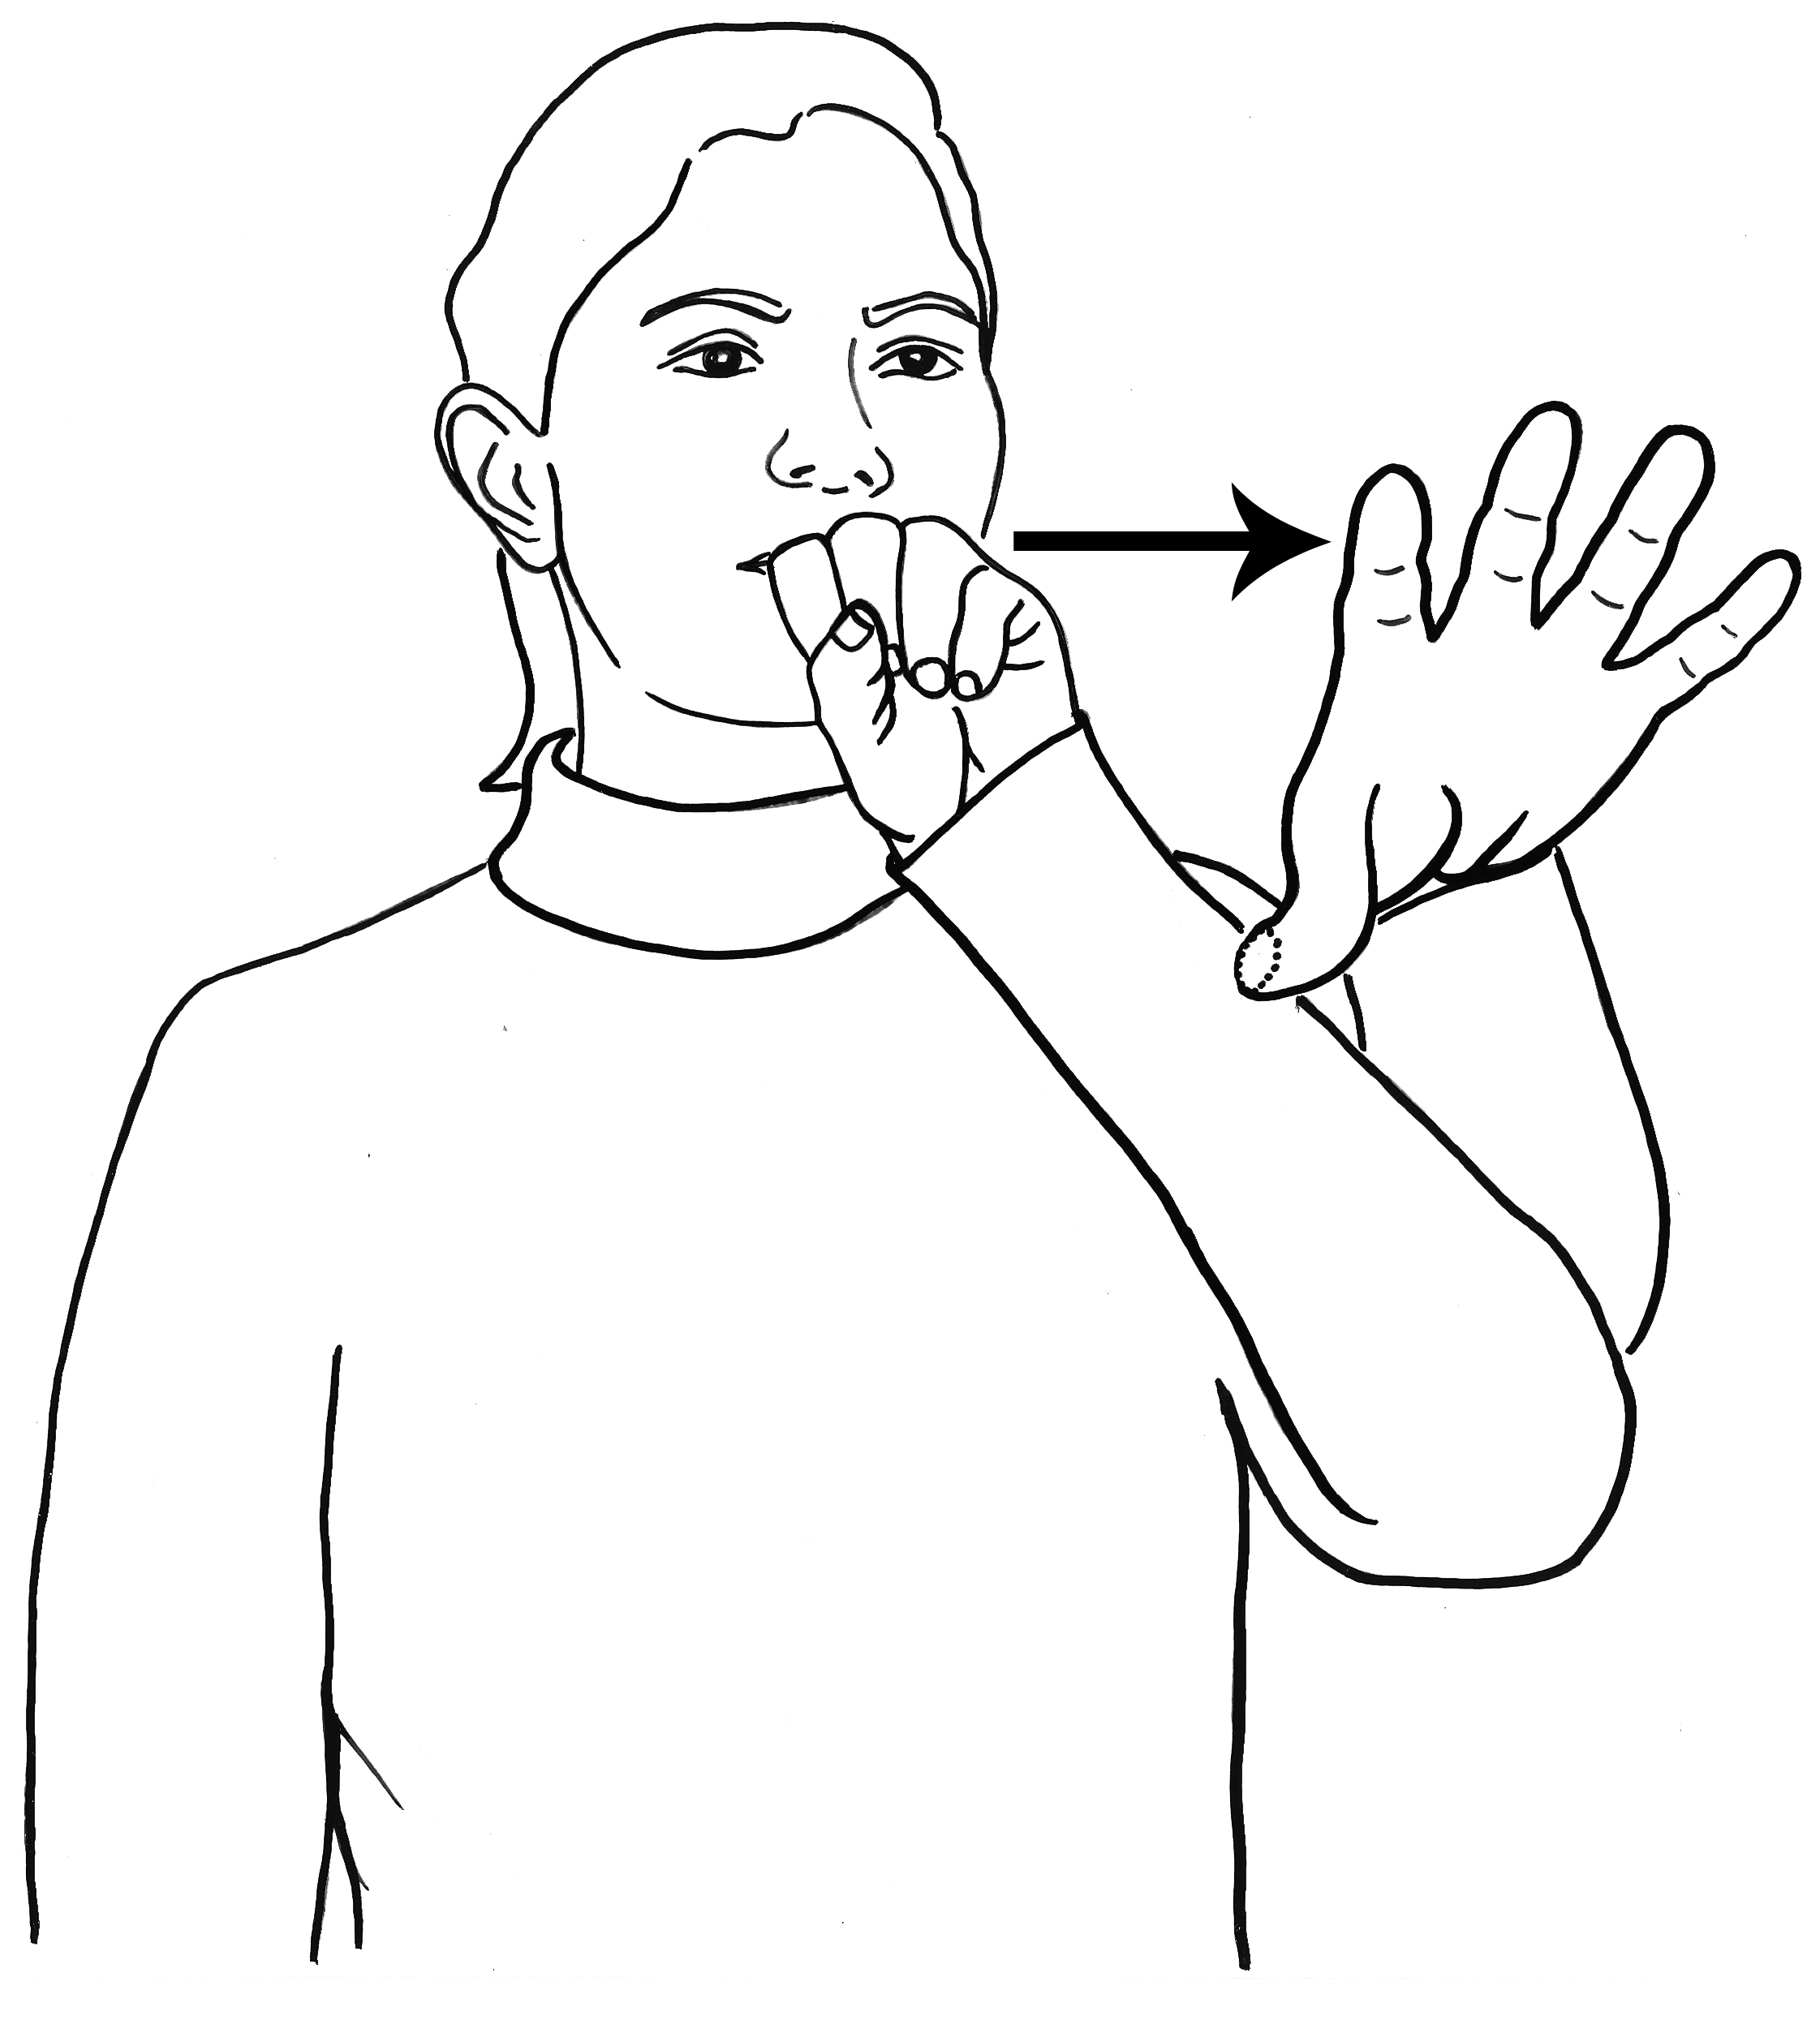
\includegraphics[width=0.32\textwidth]{figures/1b__TATTLE.jpg}}
\caption{Minimal pair in \ili{Israeli Sign Language} distinguished by place of articulation:  (a) SEND (torso) and (b) TATTLE (head)}
\label{fig:sandler:1}
\end{figure}


A sign in sign language roughly corresponds to a word in spoken language, bearing a conventionalized form-meaning relation, and constrained in form both phonotactically \citep{Battison1978,Mandel1981} and prosodically \citep{Sandler1999}.  Signs are typically monosyllabic, characterized by a single movement of the hands from one location to another. Even morphologically complex signs are usually monosyllabic, since grammatical morphemes are nonconcatenatively (simultaneously) overlaid on the base sign, by changes in locations, types of movement, and/or rhythm, and with particular conventionalized facial expressions \citep{Sandler1999}. %\citep[][and much subsequent work]{Coulter1982} and much subsequent work).  reference missing

At the level of phrasal prosody, manual timing establishes rhythm, and facial expression and head movement function systematically as intonation \citep{Nespor1998,Dachkovsky2013}.  To prepare for the discussion of prosody as an early feature of ABSL, a brief discussion of the way the body expresses prosody in sign languages is in order.  

\is{sign languages!established} \is{intonation} In an established sign language, the end of an intonational phrase is signaled by phrase final lengthening on the hands, coordinated with a change in facial expression and head position.\footnote{These intonational phrase markers are documented for two unrelated sign languages:  Israeli and American \citep{Dachkovsky2013}.}  \figref{fig:sandler:2} shows the boundary between the two intonational phrases in the \ili{Israeli Sign Language} sentence glossed roughly [[DOG SMALL THAT] [WEEK-AGO I FIND IT]] //  [[ESCAPE]] meaning ‘The little dog that I found last week // ran away.’\footnote{The first intonational phrase in the sentence is comprised of two lower level phonological phrases.} \figref{fig:sandler:2} shows that there is an across the board change in facial expression and head position between the end of the first constituent (...FIND IT) and the second (ESCAPE).\footnote{In the context of language typology featured in this volume, it is worth mentioning that well studied established sign languages seem to have similar articulator-to-linguistic function correspondence to that shown in \figref{fig:sandler:3}, and thus constitute a language type.}

\newcolumntype{L}[1]{>{\raggedright\let\newline\\\arraybackslash\hspace{0pt}}m{#1}}
\begin{figure}
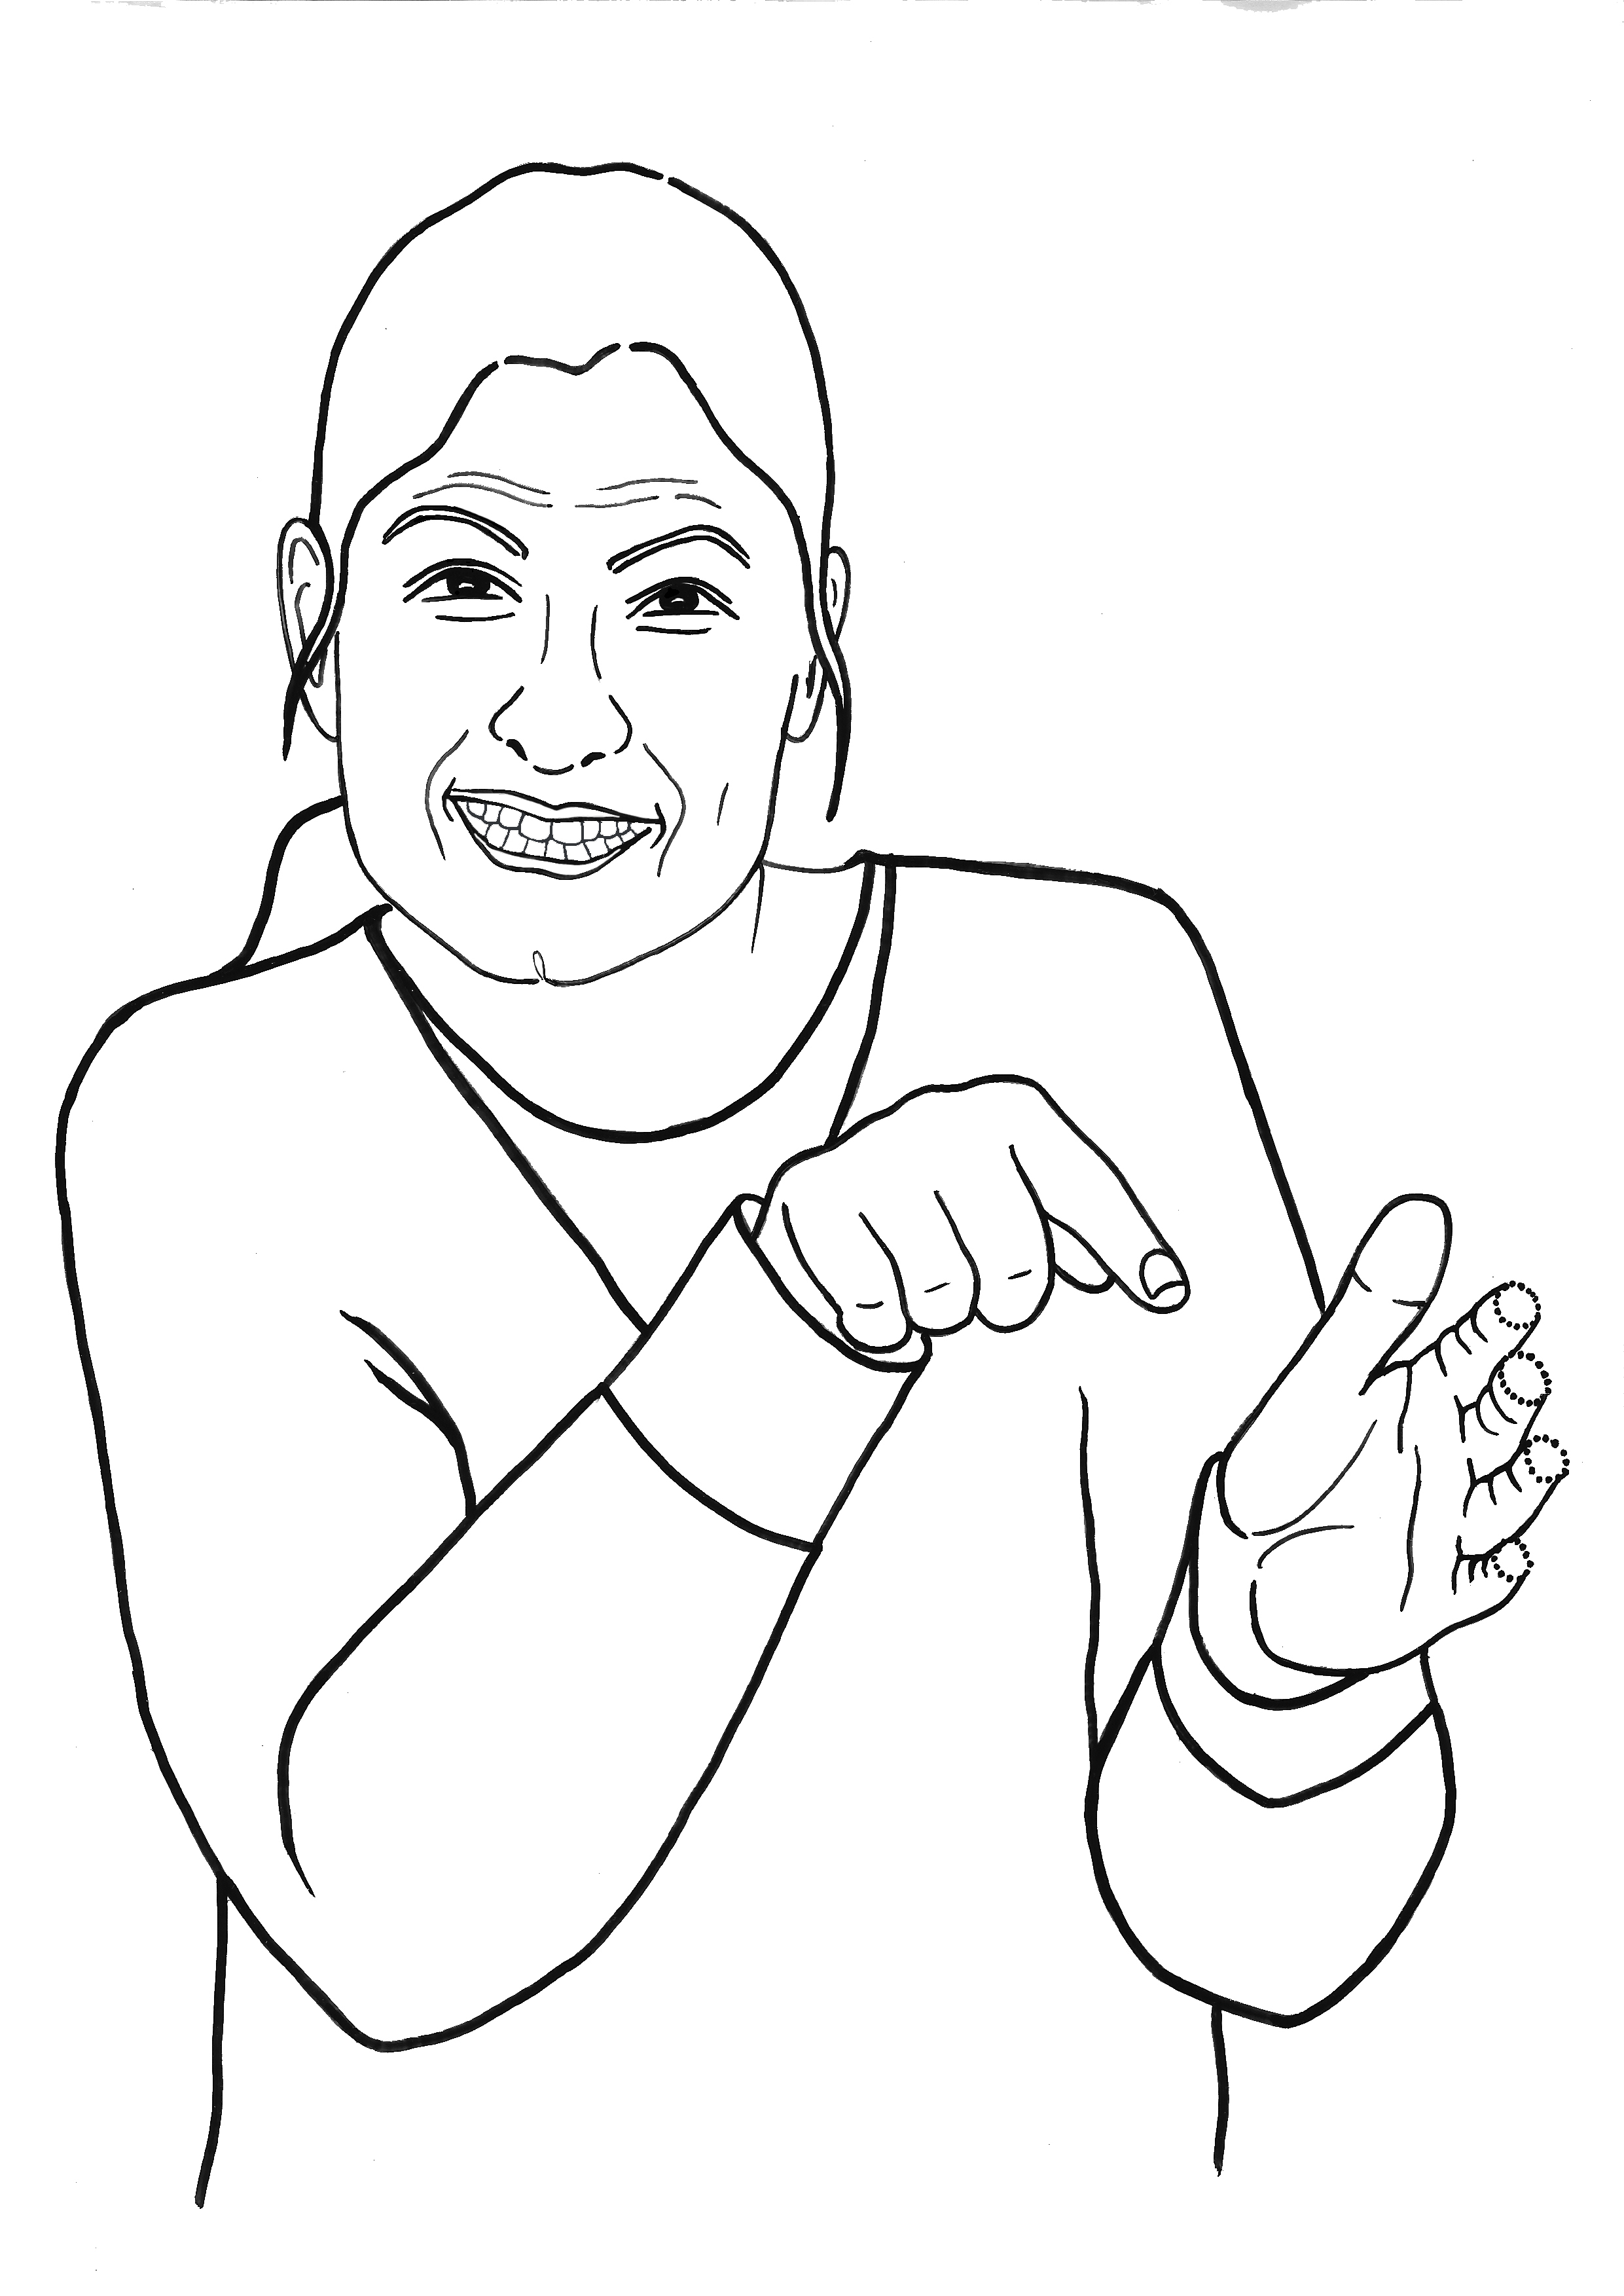
\includegraphics[width=0.32\textwidth]{figures/2a__IT_.jpg}
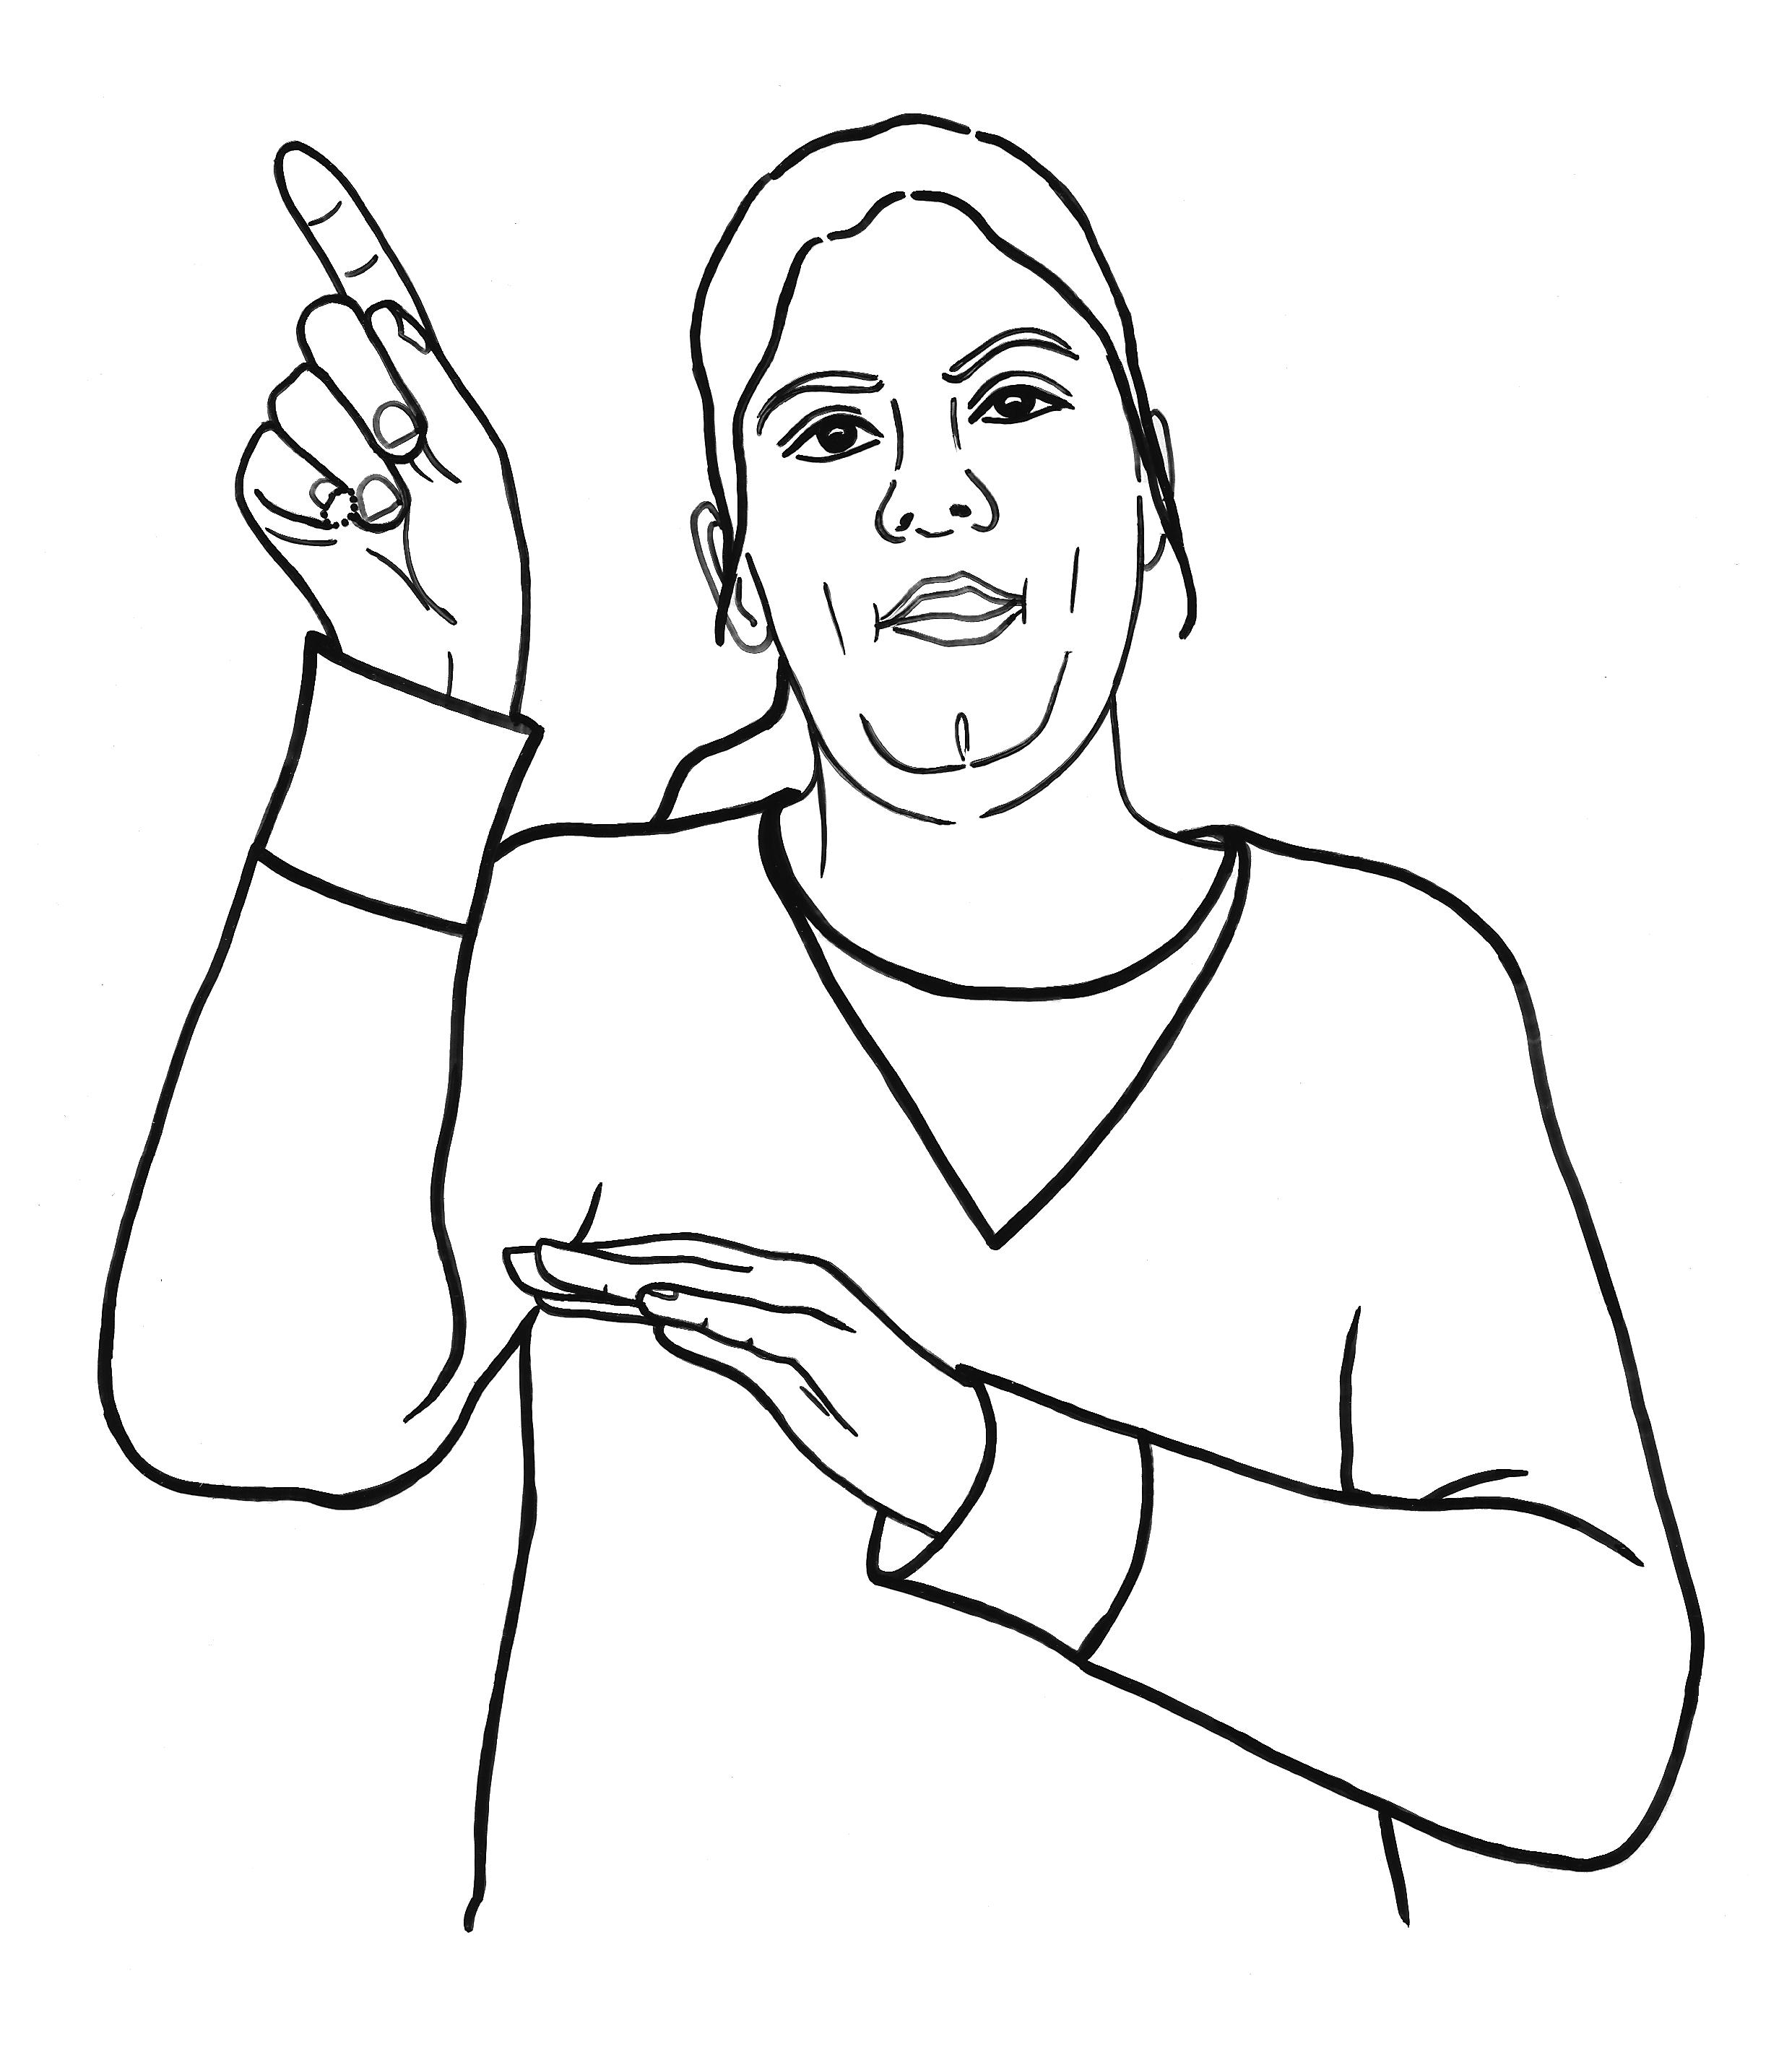
\includegraphics[width=0.38\textwidth]{figures/2b__ESCAPE.jpg}
\caption{Complete change in facial expression and head position at intonational phrase boundary between (a) [[…IT]] and (b) [[ESCAPE]] i.e., between the topic, 'The little dog that I found a week ago,' and the comment, 'ran away'.}
\label{fig:sandler:2}
\end{figure}
\newcommand{\tabitem}{~~\llap{\textbullet}~~}

\begin{figure}
\begin{tabular}{L{\textwidth}}
{ }\\
\multicolumn{1}{c}{\textbf{(a)}}\\
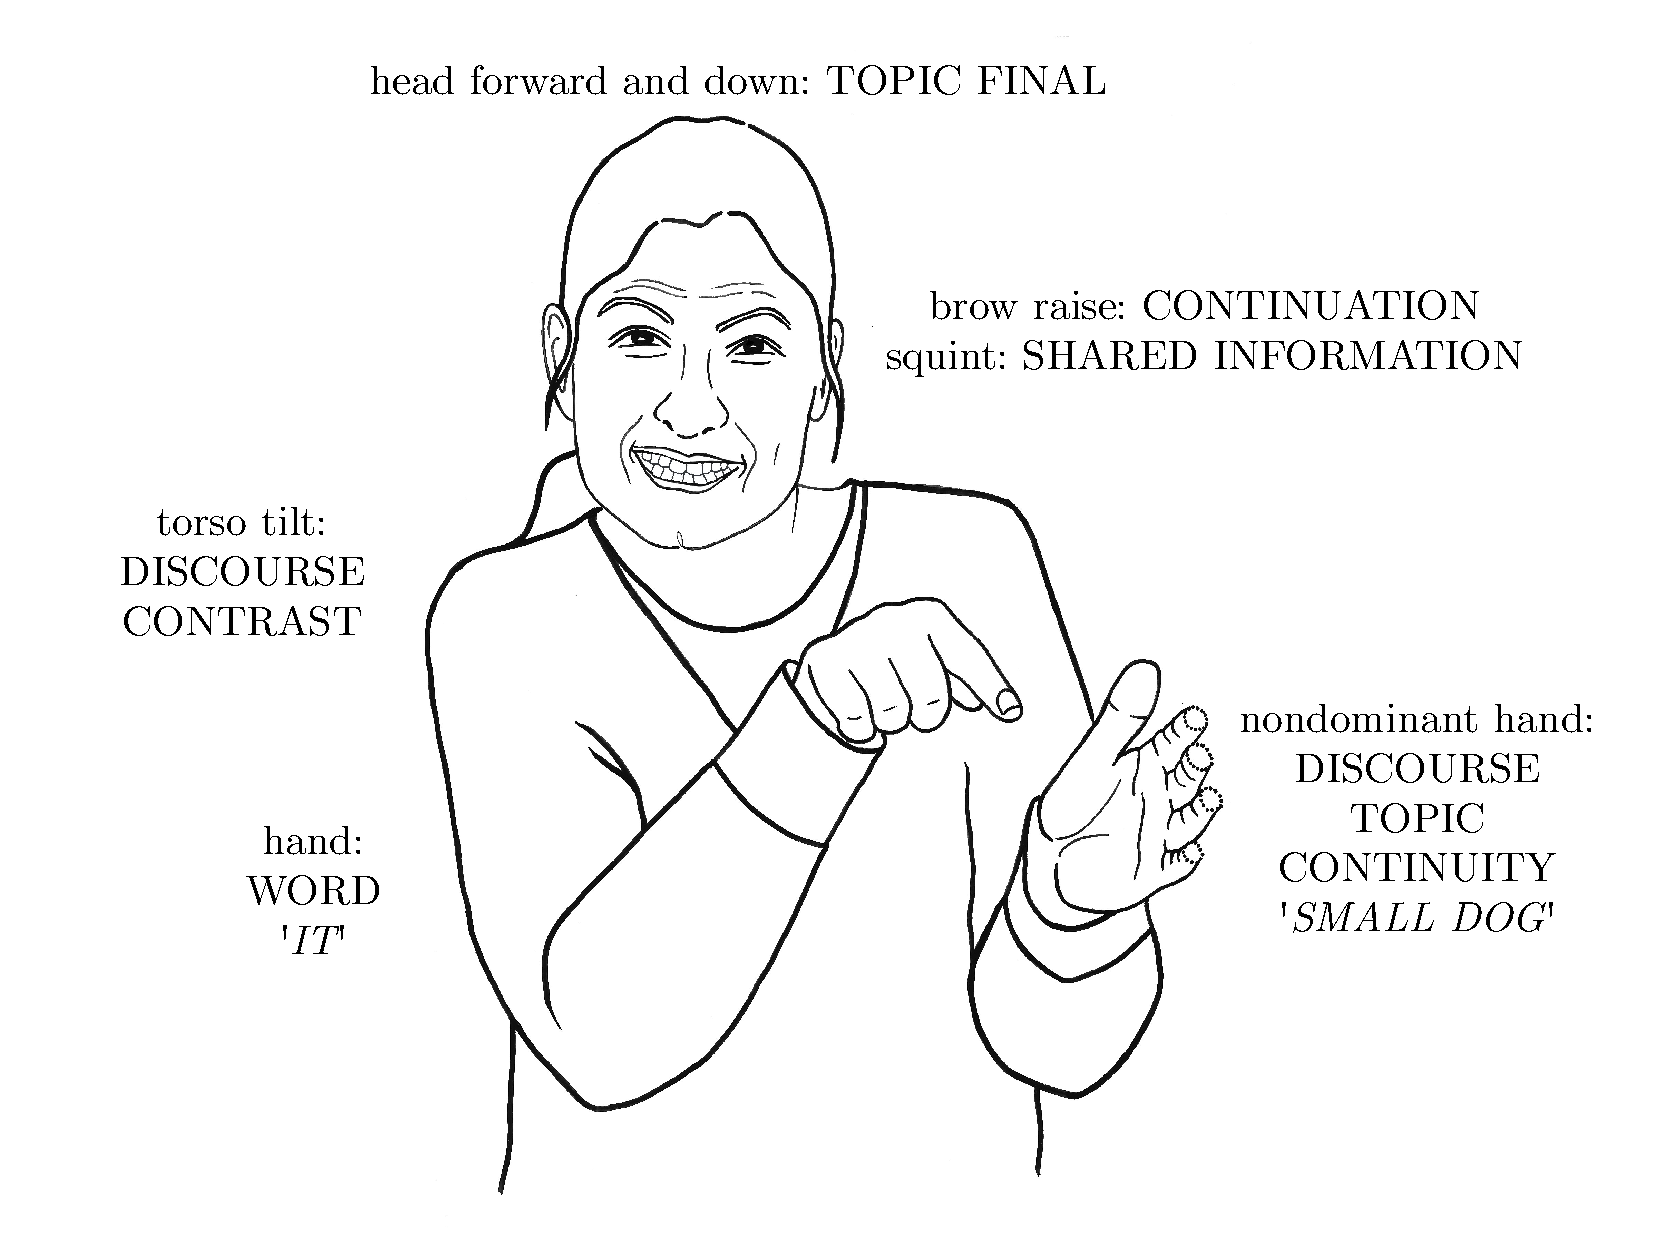
\includegraphics[width=\textwidth]{figures/sander-grammar-of-the-body-REVISED.pdf}\\
\hline
{ }\\
\multicolumn{1}{c}{\textbf{(b)}}\\
\tabitem \footnotesize \textbf{Eyeballs}: gaze (pointing; questioning; referential shift)\\
\tabitem \footnotesize \textbf{Head}: topic marking; question marking; prominence; continuation/dependency; referential shift; constituent boundary marking\\
\tabitem \footnotesize \textbf{Upper Face (brows, lids, cheeks)}: utterance type and information status (questions; old information; focus, etc.); constituent boundary marking (with blink); character perspective\\
\tabitem \footnotesize \textbf{Lower Face (tongue lips, cheeks)}: adj., adv. modification; mouthing of spoken words\\
\tabitem \footnotesize \textbf{Torso}: referential shift; discourse contrast\\
\tabitem \footnotesize \textbf{Hand(s)}: words (phonology; morphology); rhythm; prominence; boundary strength\\
\tabitem \footnotesize \textbf{Nondominant Hand}: phonological element in words; independent classifier morpheme; discourse topic continuity\\
{ }\\
\end{tabular}
\caption{(a) Functions signalled by movement of articulators at the end of the topic constituent. (b) list of functions signaled by various articulators in the language generally.}
\label{fig:sandler:3}
\end{figure}

\is{shared information} \is{topic} In this sentence of ISL, the dependency between the two constituents is indicated by raised brows and head forward and down at the end of the first major constituent, the sentence topic, and by an across the board change of face and head configurations for the second, the comment.  Squinted eyes indicate shared information – the little dog that the signer and addressee know about – a reliable signal for relative clauses \citep{Nespor1998,Dachkovsky2009}. The nondominant hand retains its shape and position from ‘small dog’ throughout the first constituent (through ‘find it’), signaling topic continuity.  This means that the anaphoric pronoun ‘it’ and the topic antecedent ‘small dog’ overlap temporally in the signal, as do the intonational and rhythmic markings of prosodic structure. In Figure 3a, a close-up of Figure 2a, the articulators are labeled for the specific functions they convey at the end of the first constituent.  Figure 3b lists some of the linguistic functions conveyed by movements of articulators in the language generally. This complex simultaneous layering of bodily signals systematically organizes information in sign language sentences \citep{Wilbur2000}.  We can now turn to the order of emergence of the two pairs of structures of interest here: words and phonology, and prosody and syntax. \is{words vs. phonology} \is{prosody vs. syntax}

\is{Pidgins} In the case of words, it is commonly believed that it would not be possible to amass a large vocabulary with holistic signals, and that a lower level of recombinable meaningless units (i.e., phonology) must have been a prerequisite for a large lexicon \citep{Hockett1960,Pinker2005}.  As for prosody, two competing predictions can be put forward, either prosody and then syntax or syntax and then prosody.  Specifically, it has been hypothesized that, in a young language, such as a pidgin, prosody might precede syntactic marking to indicate different sentence types and subordination \citep{Givón1979}. \is{subordination} On the other hand, synchronic linguistic theory typically points in the opposite direction, holding that prosodic constituents are projected from syntactic constituents \citep{Selkirk1984,Nespor1986}. \is{synchrony}

\newpage 
It is striking that neither in the case of words/phonology nor of prosody/syntax, do these paired elements appear at the same time in ABSL.  Instead, one precedes the other:  the language accrues a relatively large lexicon before phonological structure crystallizes, and prosodic markers of relations such as coordination and dependency between propositions appear in the absence of identifiable syntactic marking of these relations.  While there is already evidence for the beginnings of phonology, there is in fact very little in the way of overt syntax even in third generation ABSL signers.   

\section{Words first, phonology later}

We have followed the emergence of ABSL by recording and analyzing the language of people of different ages in the village.  This investigation reveals that the word is the first linguistic unit to appear, and that this symbolic pairing of form and meaning is at the heart of human language \citep{Sandler2013}.  Zooming in to the structure of words in an emerging language shows a considerable amount of variation as well as the beginnings of structure.  \is{emerging languages}

\subsection{Lexical form}

Our earliest data consist of a videotaped story told by an elderly man who was one of the first four deaf children born into one family in the village.  His utterances consist mainly of a series of one or two word-like manual signs, e.g., RIFLE, or HORSE RUN, occasionally interspersed with pantomimic movement of the whole body, e.g., ‘strike-with-sword’.\footnote{Pantomimic use of the body means that the body represents a human body performing some action: the hands are hands; the head is a head; the torso is a torso.  }\textsuperscript{,}\footnote{Some utterances in the narrative have more words in a constituent, including what might be analyzed as a complex sentence or two.  However, the majority of utterances are minimal, and often vague, as exemplified here.} 

\is{sign languages!established} Restriction of linguistic form to the hands is in stark contrast with the linguistic uses of the body schematized in \figref{fig:sandler:3}.  Given the availability of the whole body, and the complex and systematic use of different parts of the body in established sign languages, it is striking that only the hands are used for linguistic function at the beginning of language \citep{Sandler2012a}, to symbolize word-level concepts.  

\is{linguistic complexity} In fact, the language used by this first generation signer is as simple and vague as the content of his story is detailed and complex, suggesting that a high level of cognitive complexity is possible without a concomitant degree of linguistic complexity.  The story comes from the history of Al-Sayyid, and was translated for us by the man’s hearing son, who filled in a good deal of information shared by members of the community which was necessary for understanding the story but was not overtly conveyed.   

\is{familylect} \is{iconicity} \is{lexeme formation} Studying vocabulary in ABSL generally, we were surprised to find quite a lot of variation in lexical items across this small community, with more convergence within families, prompting us to coin the term, ``familylect".  Certain patterns can be identified at the level of the word, such as iconically motivated regularities in lexeme formation \citep{Padden2013,Lepic2016}.  The only evidence we have found of complexity at the word level is in the formation of compounds, which show considerable variation in structure, with the exception of a language-particular subset involving classifier morphemes that typically follow a noun \citep{Meir2010,Sandler2011a}. \is{classifiers}


\subsection{Articulatory variation: no crystallized phonological system}

In our investigation of sign production across the community, we also found a surprising amount of articulatory variation in the production of the same lexical item %\citep{Israel2011} reference missing
\citep{IsraelSandler2011}.   In this way, the words of ABSL are unlike the words of more established sign languages because they function as iconic wholes, and we concluded that a phonological system has not yet crystallized across the community \citep{Sandler2011a}.

Our team created a dictionary with 300 entries, presumably only a fraction of the lexicon in the language, since the signs had mostly been elicited through picture naming and the majority are thus concrete nouns.  Yet, despite a relatively large vocabulary, we could not detect evidence of a discrete, systematic, meaningless level of structure. Even broad phonological specifications in established sign languages, such as major place of articulation categories, on a par with LABIAL or DORSAL in spoken languages, varied across signers for the same sign, as exemplified in \figref{fig:sandler:4} for the sign DOG.  The two places of articulation shown here, head and torso, are major place categories and contrastive in more established sign languages (cf., SEND and TATTLE in ISL, \figref{fig:sandler:1}).   \is{sign languages!established}

\begin{figure}
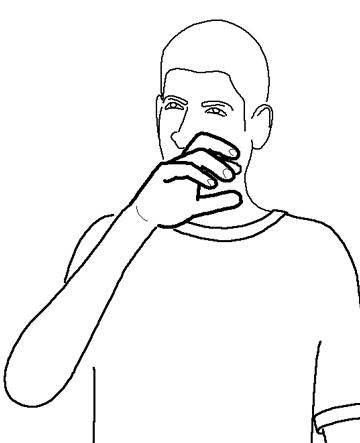
\includegraphics[width=0.32\textwidth]{figures/4a_DOG__face_.jpg}
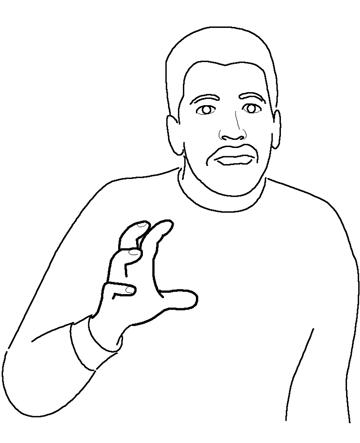
\includegraphics[width=0.32\textwidth]{figures/4ba__DOG__torso_.jpg}
\caption{The ABSL sign DOG signed by different signers at two different places of articulation, the head (a) and torso (b). The same two places of articulation are contrastive in established sign languages (see Figure 1).}
\label{fig:sandler:4}
\end{figure}

\is{ease of articulation} \is{iconicity} \is{familylect} We did discover kernels of phonology. For example, we encountered signs among younger signers whose form had been consistently altered to accommodate ease of articulation, resulting in signs that are counter-iconic.  This suggests that smaller units of meaningless form are taking precedence over iconic, holistic signals. Within what we dubbed a ``familylect", we also found consistent form-based handshape assimilation in a frequently used compound rendering it, too, non-iconic, and suggesting the beginning of a phonological level \citep{Sandler2011a,Sandler2014nordlyd}.  We deduce from these studies that the emergence of phonology, at least in a contemporary sign language, depends first on the conventionalization \is{conventionalization} \is{automacity} of words and then on frequency of use and automaticity.  The answer to the empirical question of how many meaningful holistic signals humans can produce and perceive in the vocal/auditory modality is not known, and it is possible that sign languages can tolerate a larger number than spoken languages can, due to the iconicity of form and the nature of visual perception.  But even if there is some difference between modalities in this regard, ABSL shows surprisingly that it is possible for a functioning human language to have a relatively large vocabulary without a crystallized phonological system, making phonology dependent, in the sense intended here, on a stable, conventionalized, and frequently shared lexicon. \is{iconicity} 

\section{Prosodic organization first, syntax later}

\is{rhythm} \is{intonation} \is{phrasal stress} How are these words combined into meaningful utterances?  In established languages, prosodic signals – rhythm, intonation, and phrasal stress -- are typically coextensive with syntactic constituents such as the phrase or the clause.  It has been argued that phrasal stress is determined by the order of heads and complements in a language \citep{Nespor1986}, and that children, sensitive to prosody of their native language since infancy \citep[e.g.,][]{Mehler1994,Juscyk1997}, use the prominence patterns of prosody to bootstrap the syntactic structure \citep[e.g.,][]{Nespor1996}.  

Because of this syntax-prosody correspondence, linguists propose that the prosody is read off the syntax, and is in this sense dependent on it \citep{Selkirk1984,Nespor1986}.  Given these observations, one might expect syntactic structure to be a prerequisite for prosodic structure in a new language.  This prediction runs contrary to that of \citet{Givón1979} and others who reason that prosody is likely to precede syntax in young languages.

\is{syntax} \is{word order} \is{autonomous syntax} \is{human vs. inanimate} The difference between these two views may depend to some extent on what one calls syntax.  Our approach throughout has been to refrain from attributing autonomous syntactic form to an expression in ABSL without explicit evidence for it.\footnote{Apart from overt markers, syntactic tests can identify syntactic structure.  For example, early research on American Sign Language distinguished coordinate from subordinate clauses by the coreference properties of a process called final subject pronoun copy \citep{Padden1988}.  In ABSL we have not found syntactic processes of this kind, nor do we see evidence of morphosyntax, such as verb agreement \citep{Padden2010}, although it is common in established sign languages \citep{Aronoff2005}, or case marking.  While one cannot rule out the covert presence of syntactic structure driving the prosodic structure we see, neither can we identify evidence for its existence.  The more parsimonious account, therefore, is one that takes prosody as the prior mechanism for organizing and relating essentially semantic constituents.}  We find word groupings by meaning and even consistencies in word order \citep{Sandler2005}, but no evidence so far that favors autonomous syntactic structure over a much more basic driving force.  In a recent and detailed study, \citet{MeirSubmitted} show that word order in new sign languages and in gesture (without speech) is governed by the salience of human referents and not by syntactic rules.\footnote{Based on word orders of ABSL and other new sign languages, and on experimental work with gesture, \citet{MeirSubmitted} found that human arguments occur before inanimate arguments, irrespective of their syntactic or semantic roles.}  In ABSL, the groupings of words into constituents and the relations between them are marked by prosody, which emerges gradually over time in the community \citep{Sandler2011b}.

\is{syntactic relations} On the whole, evidence from a small sample of narratives in four ABSL age groups suggests that prosody – consisting of timing and intonation -- is the earliest organizing force, and that it emerges gradually.  This overall picture is tempered by the fact that certain indications of syntactic relations \textit{within} clauses begin to appear together with intonational marking of dependency \textit{across} them. The findings are summarized in Tables 1 and 2. We are currently investigating these preliminary results further, across three young sign languages.



\begin{table}

 \begin{tabular}{cccccc}
\lsptoprule
  Age group & Hands & Head & Face & Body & Nondominant hand \\
\midrule
 1 & × & { } & { } & { } & { } \\ 
 2 & × & × & { } & { } & { } \\
 3 & × & × & × & { } & { }\\
 4 & × & × & × & × & × \\
 \lspbottomrule
\end{tabular}
  \caption{Recruitment of additional articulators for grammatical functions according to age group, from oldest (group 1, the earliest stage of the language) to youngest (group 4, the later stage)}
   \label{tab:sandler:1}
\end{table}

\usepackage{array}
\newcolumntype{x}[1]{>{\raggedright\arraybackslash\hspace{0pt}}p{#1}}

\begin{table}

\begin{tabular}{x{0.1\textwidth}x{0.08\textwidth}x{0.4\textwidth}x{0.28\textwidth}}
\lsptoprule
Age group & Words & Complex sentences & Discourse/reference cohesion\\
\midrule
1 & Signs & { } & { } \\
2 & Signs & Unsystematic clause linking (coordination); 1 NP per 2.5 predicates (vague one-word constitutents); 1st person subject pronouns only & { } \\
3 & Signs & Many dependent constituents (conditionals, temporal expressions, reported speech); 1-2 NPs per predicate; 3rd person pronouns & Parentheticals, reported speech \\
4 & Signs & Addition of modifiers, quantifiers, embedding inside reported speech (double embedding) & Addition of topic continuity marker and torso shift for different discourse referents\\
\lspbottomrule
\end{tabular}
\caption{Complexity added through recruitment of additional articulators for linguistic functions \citep[adapted from][]{Sandler2011b,Sandler2012a}}
\label{tab:sandler:2}
\end{table}


\textbf{Age group 1}.  As I pointed out in the introduction, the story told by the oldest signer (age group 1), is characterized largely (though not exclusively) by one or two-word propositions, separated by pauses.  Only the \textit{hands} are recruited for linguistic components.  

\textbf{Age group 2}.  In the second age group (short stretches of narratives of two people in the study reported in \citealt{Sandler2011b}), movement of the \textit{head} was added to the hands to separate constituents.  Some separated constituents were lists, and some (e.g., temporal expressions such as DAYS THREE meaning ‘for three days’) were related semantically to adjacent propositions, but no special syntactic or prosodic marking distinguished these from coordinated units.  Many propositions in this age group did not associate nominal arguments with verbs in the same constituent, and no pronouns were used except occasionally first person (pointing to the chest).  

\is{conditionals} \is{parentheticals} \is{subordination} \textbf{Age group 3}.  In the third age group (short stretches of narratives of two younger people), \textit{facial expression} was added to show continuation/dependency between constituents such as conditionals, and, together with head position, to signal parentheticals in a discourse.  Although utterances clearly involve subordination semantically (e.g., in conditionals), this subordination is not marked syntactically – no complementizers, time adverbials, or conditional expressions like ‘if’.  Instead it is marked with prosodic signals of timing of the hands and intonation of the face and head.  \is{complementizers} \is{time adverbials}

Together with prosodic signaling of dependency between clauses, we see somewhat richer structure within clauses:  verbs are more likely to occur with nominal arguments, and third person pronouns -- abstract syntactic elements -- are common.  Relations between clauses are signaled prosodically by timing and intonation, and not syntactically, but a tendency that might be considered syntactic is emerging:  an increase in overt arguments associated with verbs, some of them pronominal forms. We see no implicational relation between these syntactic elements within clauses and the prosody connecting them, however.  

While we cannot rule out the covert presence of syntactic structure driving the prosodic structure we see, neither can we identify evidence for its existence.  The more parsimonious account, therefore, is one that takes prosody as the prior mechanism for organizing and relating essentially semantic constituents.  We conclude that the mechanism for connecting clauses and indicating dependency relations between them is prosodic, and that syntactic mechanisms serving this function have not (yet) arisen.  For further discussion of what you can say without syntax, see \citegen{Jackendoff2014} paper with that title. 
 
\largerpage[-1] 
\textbf{Age group 4}.  We are just beginning to analyze the language of age group 4.  The narrative of a single signer in the fourth age group was chosen for analysis for two reasons:  he is the oldest of five deaf siblings in one household and his deaf mother and hearing father know only ABSL and no ISL,\footnote{The young people of the Al-Sayyid village have had a good deal of exposure to signs from \ili{Israeli Sign Language} in school settings, while exposure to ISL grammatical structure as it is signed by deaf people is limited.  In school, the teachers speak \ili{Arabic}, accompanied by ISL signs. This is not ISL, since the grammar of the sign language is very different from that of the spoken language, and, as with other sign-supported speech systems, when both channels are used at the same time, one or the other (usually the sign language) is seriously disrupted.  Some of the young deaf men in Al-Sayyid (including the Group 4 example discussed here) did have extended exposure to ISL in their late teens when they attended a mixed vocational high school (Jewish and Arab pupils with ISL signing deaf teachers), now closed down. The bottom line is that people under the age of 30 have had considerable exposure to ISL vocabulary and sporadic, uneven exposure to its grammatical structure.  A general description of the spoken and signed linguistic mosaic in Israel is offered in \citet{Sandler2014nordlyd}.} so that the young man is able to distinguish the two languages and provide a good example of ``pure", fluent ABSL in his age group.

In his signing we found refinement and coordination of the nonmanual signals for subordination/dependency (cf. ISL example in \figref{fig:sandler:3}).  Even double embedding of constituents occurs.  An example is an utterance translated (with the help of prosody) as, “Father (said to) me about marriage, ‘If you marry a deaf girl, all of your children will be deaf.  No way.’” The boldface constituent in the gloss has conditional prosody: FATHER ME MARRIAGE, \textbf{DEAF TWO DEAF BOTH MARRY}, OFFSPRING DEAF ALL – REJECT.  As with age group 3 signers, this embedding of one proposition within another is signaled by prosody only and not by overt morpho-syntactic elements such as a conditional word like 'if'. \is{embedding} 

\is{topic} \is{coreference} \is{discourse} In his narrative, the signer added the \textit{nondominant hand} for topic continuity (essentially, discourse level coreference) and shifts in \textit{body posture} to identify referents in a discourse.  All of these phenomena are structural advances over the narratives of the earlier stages of the language of the older people studied.  \tabref{tab:sandler:signer's narrative} is a gloss and translation to \ili{English} of an excerpt in which he describes the vocations (professions) he had to choose from at vocational school. A parenthetical segment is set off in the gloss by square brackets.  The large curly bracket along the side indicates the stretch of signing during which the nondominant hand is held in the signal to mark continuity of the topic -- ‘the third vocation’ (welding) -- dropping to his side at the end of the discourse segment relating to the topic. \figref{fig:sandler:6} illustrates the physical manifestation of linguistic properties of the utterance.  The signer’s budding Grammar of the Body \is{grammar of the body} may not yet be as systematic and complex as that of more established sign languages, \is{sign languages!established} but it has the scaffolding in place. 

\begin{table}
\begin{tabular}{rlL{0.5\textwidth}}
\lsptoprule
&Gloss&Translation\\
\midrule
% &&\\
% &						&						[[One, cooking, two, mechanics, three, welding.\\
% &                       &                       \\
% &                       &                       \multirow{4}{0.5\textwidth}{[Long ago, when I was small, my father was a welder. I remembered it well and didn't want that, not welding.]}\\
% &                       &                       \\ 
% &                       &                       Four computers, all the professions.]]\\
% &                       &                       \\ 
% &                       &                       I wanted mechanics.\\
\ldelim\{{9}{5pt}[]&	ONE COOKING				& 					\multirow{3}{0.5\textwidth}{[[One, cooking, two, mechanics, three, welding.}\\
&						TWO MECHANICS			&					\\
&						THREE WELDING			&					\\
&						{[}I LONG-AGO I SMALL	&					\multirow{4}{0.5\textwidth}{[Long ago, when I was small, my father was a welder. I remembered it well and didn't want that, not welding.]}\\
&						FATHER ME HE WELD		&\\
&						REMEMBER WELL			&\\
&						NOT, REJECT]			&\\
&						FOUR, COMPUTERS			&					\multirow{2}{0.5\textwidth}{Four computers, all the professions.]]}\\
&						ALL PROFESSIONS			&\\
&						&						\\
&						ME MECHANICS.			&					I wanted mechanics.\\
\lspbottomrule
\end{tabular}
\caption{Excerpt from 4th age group signer’s narrative \citep[from][]{Sandler2012a}}
\label{tab:sandler:signer's narrative}
\end{table}

\begin{figure}
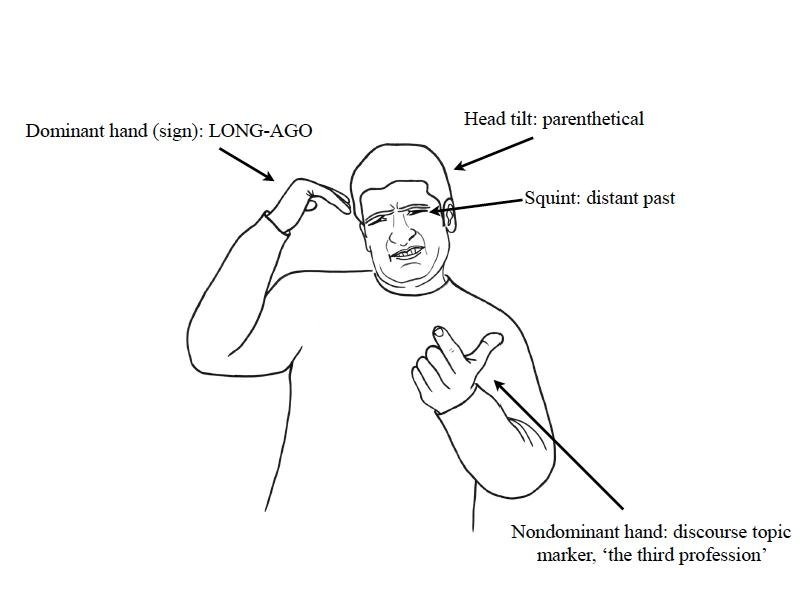
\includegraphics[width=\textwidth]{figures/6__use_of_body_ABSL.jpg}
\caption{Use of the body for grammatical functions \citep[from][]{Sandler2012a}.}
\label{fig:sandler:6}
\end{figure}



\section{Conclusion}

From a grammatical point of view, ABSL across the community is relatively simple. Nevertheless, the semantic/cognitive conceptualization and relations it reflects are far from simple.  With these conceptualizations and relations, and minimal linguistic machinery, ABSL functions as a full language.  Its users talk about life histories, folk remedies no longer in use, dreams, fertility, deafness, national insurance, wedding preparations, suspicions, personal relations – all fluently, without hesitation or pantomimic ``acting out", and without noticeable communication failures.  While further grammatical structures may develop over time, it seems that fully functional language is possible with relatively simple linguistic structure (see \citealt{Klein1997,Gil2005,Jackendoff2014} for more support for this claim).

ABSL and other new languages provide novel evidence for theories about the relation between community structure and language structure \citep{Meir2012}.  For example, the language of age groups 1 and 2 corresponds to \citegen{Bernstein1971} notion of a restricted code used in circumstances where the speakers share knowledge and assumptions.  A restricted code is economical in that it can convey a good deal of meaning with a few words, as speakers can rely on the shared knowledge of their interlocutors to interpret what they say. \is{restricted code} \is{shared information}

\is{esoteric code} We have reported elsewhere that tolerance of irregularity, in the form of lexical variation and variation in the order of constituents in compounds in the Al-Sayyid village, reported in \citet{Meir2010}, is compatible with \citegen{Wray2007} conception of an esoteric code.  Acquired in childhood and used within a homogeneous group with shared culture and environment, esoteric codes are characterized by irregularities of form that are less typical of more regular exoteric codes, used with outsiders.\footnote{As a very young language, ABSL has not had a chance to develop characteristics attributed to esoteric codes such as morphophonemic alternations and irregular morphological paradigms.  } 

The overview presented here suggests that the emergence of a crystallized phonological system follows -- in other words, depends on -- the prior existence of a sizable, conventionalized lexicon.  As for the emergence of prosody and syntax, our findings suggest that an autonomous syntax is not a prerequisite for prosody, or, in other words, that prosody does not depend on syntax.  Prosody is a critical factor in organizing semantic relations relatively early in a language, while overt indications of syntax have yet to emerge.  Language needs this basic scaffolding of words and prosody, which emerges gradually over a few generations, and it seems that it is all the linguistic machinery you need for a perfectly good human language. %In the context of evolution, let’s take a step back and consider this basic scaffolding:  symbolic words, semantically related word groupings, intonational linking of propositions.  
Simple maybe, compared to millennia-old languages.  But no other species even comes close.  

\section*{Acknowledgements}
The research on ISL is supported by grant 580/09 from the Israel Science Foundation to Irit Meir and the author. The ABSL research is supported by a grant from the U.S. Israel Binational Science Foundation and by NIH grant R01 DC006473.  The Grammar of the Body project is supported by a grant to the author by the European Research Council, project 340140.  Many thanks to Nick Enfield and other participants for useful and stimulating discussions at the meeting on Dependencies among Systems of Language, Ardennes, June 2014.  I am grateful to Mark Aronoff, Ray Jackendoff, and Keren Rice for their insightful comments and suggestions on this paper. 

{\sloppy
\printbibliography[heading=subbibliography,notkeyword=this]
}

\end{document}
